\documentclass{article}

% if you need to pass options to natbib, use, e.g.:
%     \PassOptionsToPackage{numbers, compress}{natbib}
% before loading neurips_2021

% ready for submission
\usepackage{neurips_2021}

% to compile a preprint version, e.g., for submission to arXiv, add add the
% [preprint] option:
%     \usepackage[preprint]{neurips_2021}

% to compile a camera-ready version, add the [final] option, e.g.:
%     \usepackage[final]{neurips_2021}

% to avoid loading the natbib package, add option nonatbib:
%    \usepackage[nonatbib]{neurips_2021}

\usepackage[utf8]{inputenc} % allow utf-8 input
\usepackage[T1]{fontenc}    % use 8-bit T1 fonts
\usepackage{hyperref}       % hyperlinks
\usepackage{url}            % simple URL typesetting
\usepackage{booktabs}       % professional-quality tables
\usepackage{amsfonts}       % blackboard math symbols
\usepackage{nicefrac}       % compact symbols for 1/2, etc.
\usepackage{microtype}      % microtypography
\usepackage{xcolor}         % colors
\usepackage{graphicx}

\title{ELEC 573 Project: Predicting Recurrent Stroke}

% The \author macro works with any number of authors. There are two commands
% used to separate the names and addresses of multiple authors: \And and \AND.
%
% Using \And between authors leaves it to LaTeX to determine where to break the
% lines. Using \AND forces a line break at that point. So, if LaTeX puts 3 of 4
% authors names on the first line, and the last on the second line, try using
% \AND instead of \And before the third author name.

\author{%
  David S.~Hippocampus\thanks{Use footnote for providing further information
    about author (webpage, alternative address)---\emph{not} for acknowledging
    funding agencies.} \\
  Department of Computer Science\\
  Cranberry-Lemon University\\
  Pittsburgh, PA 15213 \\
  \texttt{hippo@cs.cranberry-lemon.edu} \\
  % examples of more authors
  % \And
  % Coauthor \\
  % Affiliation \\
  % Address \\
  % \texttt{email} \\
  % \AND
  % Coauthor \\
  % Affiliation \\
  % Address \\
  % \texttt{email} \\
  % \And
  % Coauthor \\
  % Affiliation \\
  % Address \\
  % \texttt{email} \\
  % \And
  % Coauthor \\
  % Affiliation \\
  % Address \\
  % \texttt{email} \\
}

\begin{document}

\maketitle
\vskip -0.2in

\begin{abstract}
\vskip -0.1in
  Recurrent stroke incidence drastically increases a stroke patient's mortality rate, so developing a method to predict the risk of recurrent stroke is an important step towards saving lives. Therefore, I explore the application of graph learning methods to the prediction of recurrent stroke risk using medical data. Specifically, I demonstrate that HORDE, a recent graph-based representation architecture, is effective for this task using a comprehensive database of stroke patients treated in the Texas Medical Center. I also evaluate the model's ability to predict recurrent stroke based on data availability, patient characteristics, and recurrence window lengths, and report its performance with varied architectures.
\end{abstract}

\section{Introduction}

\subsection{Strokes}

As of 2015, cerebrovascular accidents, commonly referred to as strokes, are the second-highest cause of death globally, and are one of the leading causes of disease in the United States (Roth et al., 2018). Strokes occur when blood flow to the brain is disrupted, preventing the necessary amount of blood from reaching certain cells in the brain. Those who suffer strokes can lose many of the skills necessary for daily life, and usually must undergo a months-long rehabilitation process to recover these skills. However, many stroke patients cannot fully recover, and must learn to live with an impaired ability to interact with and understand the world around them (National Institutes of Health, 2019). 

\subsection{Effects of recurrent stroke}

It is estimated that over 10 million people have a stroke each year, and in 2017, strokes accounted for 11\% of deaths worldwide (Roth et al., 2018). Although the mortality rate for stroke patients is relatively low, those who have a recurrent stroke suffer a mortality rate above 50\%, making these additional strokes incredibly dangerous. In fact, whether a patient suffers a recurrent stroke is the best predictor of mortality: those who do are \textasciitilde16.7 times more likely to die within a decade of their first stroke (Aarnio et al., 2014). Understanding how to predict and mitigate recurrent strokes is therefore incredibly important to reducing patients’ rates of mortality, disability, and financial hardship. 

\subsection{Problem description}

I leverage data observed about a stroke patient during medical appointments to predict whether they will have a recurrent stroke. Given a matrix $\bold{X} \in \mathbb{R}^{T \times N}$ describing $N$ features of a patient's condition at each of $T$ timesteps, and a vector $\bold{d} \in \mathbb{R}^M$ describing $M$ time-invariant characteristics of the patient, my project will be to determine a parametrized function $f_\theta : (\bold{X}, \bold{d}) \rightarrow \left[0, 1\right]$ with parameters $\theta$ that computes the probability that the patient will have a recurrent stroke within an $m$-month window. 

\section{Related work}
\subsection{Machine learning for recurrent stroke prediction}
In recent years, machine learning has been applied to medical datasets for a variety of downstream tasks. These models typically leverage electronic health records (EHRs), which are tabular data that describes a patient's demographics, vital signs, symptoms, and other information across multiple medical visits. Although EHRs have been effective data sources for other downstream tasks, few attempts have been made to use them for predicting recurrent stroke. The most prominent papers have produced moderate results: a 2020 paper by Hung et al. leverages a Naive Bayes model to obtain an AUROC of 0.661, while a 2021 paper by Abedi et al. leverages gradient-boosted trees to obtain an AUROC of 0.69. Although these scores are decent, they are below the standard necessary for deployment to medical environments, so I hope to improve on this work using graph learning.

\subsection{Graph representation learning for medical data}
Graph-based representation has been successfully leveraged for medical prediction tasks. A 2020 paper published by Lee et al. introduced the HORDE framework, a graph-based method embedding method for medical data. HORDE enables the learning of latent embeddings for patients based on not only EHRs, but other data modalities as well, with demonstrated success using medical concepts extracted from hand-written clinical notes. Since EHRs are often inaccurate and incomplete descriptions of a patient's condition, incorporation of additional medical data modalities can improve performance. Further, HORDE accounts for temporal information by constructing a graph that varies between timesteps (called \textit{encounters}) representing successive medical visits; the resulting embeddings, computed in an unsupervised manner using graph convolutional networks (GCNs) and long-short term memory (LSTMs), describe how each patient's condition changes over time. Briefly, the HORDE graph is constructed with both patients and features as nodes, drawing edges, weighted by feature value, between patient and feature nodes at timesteps where that patient has a non-zero value for that feature. This structure enables the exchange of information between patients, EHR features, and (for example) medical concept features. Although HORDE has not been used for recurrent stroke prediction as of yet, the framework has successfully been applied to a dataset of ICU patients for both future diagnosis prediction and visit severity classification.

% \subsection{Heterogeneous graph representation learning}
% Although HORDE constructs a graph with heterogeneous nodes, its embedding method does not differentiate between modalities. Therefore, a potential area for improvement is to incorporate an embedding method that better accounts for each modality; one example is HAN, a heterogeneous graph representation model introduced in a 2019 paper by Wang et al. While traditional representation architectures do not differentiate between node modalities, HAN groups node neighborhoods into meta-paths, which each describe a distinct ordering of node modalities (e.g. Actor --- Movie --- Actor, for co-actors). This preserves the unique semantic information held within each meta-path, producing embeddings that outperform homogenous methods. 

\section{Dataset}
In working with the University of Texas Health Science Center at Houston (UTHealth) for my senior capstone, I have been granted access to a labeled database of EHRs, over up to 69 encounters, for 4,776 UTHealth hospital patients---one of the most comprehensive in the world of its kind. Each patient in the database suffered at least one stroke, and approximately 25\% of these patients suffered recurrent strokes within one year as well. The EHRs are represented in tabular form, and consist of approximately 5,000 features describing patients' demographics, along with their diagnoses, lab tests, measurements taken, and other information throughout their medical appointments. The raw text of approximately 2 million clinical notes is also included in the dataset, along around 8,000 CT and MRI scans; however, this project leverages only the EHRs, and the other modalities will be incorporated in future work.


\section{Preliminary analysis}
\subsection{Aggregated HORDE graph overview}
To confirm the validity of a graph-based approach and describe the dataset for my sponsors at UTHealth, I first performed exploratory analysis using graph-based methods. For this analysis, I leveraged a time-invariant version of the HORDE graph, ${\textbf G_{agg}}$. The input EHR data is binarized and aggregated over time, such that each edge connecting a patient-feature node pair is weighted as the total number of times that feature was measured for that patient throughout all of their hospital visits.
\begin{table}
    \caption{
      Graph-level statistics for G$_{agg}$
    }
    \label{tab:exp}
    \centering
    %
    \centering
    \label{tab:exp-synth}
    \begin{small}
    \begin{sc}
    \begin{tabular}{lrrr}
    \toprule
    Statistic                       & Value \\
    \midrule
    Nodes                         & 8068 \\
    Patient nodes                         & 3801 \\
    EHR feature nodes                         & 4267     \\
    Edges                            & 1,290,078    \\
    Mean edge weight                                  & 7.75 \\
    Mean patient node degree              & 2632.4    \\
    Mean feature node degree                   & 2345.0    \\
    \bottomrule
    \end{tabular}
    \end{sc}
    \end{small}
\end{table}

Table 1 describes several graph-level statistics of ${\textbf G_{agg}}$, which was created from an 80\% training set. It’s notable that only 8\% of possible patient-feature edges are present, meaning that, as expected, the EHR dataset is relatively sparse and therefore suitable for graph-based analysis. Also, based on the high mean edge weight, patient-feature pairs that are measured are generally sampled across many encounters, indicating the presence of temporal information that can likely improve modeling performance.

\subsection{Node centrality}
I also examined the weighted degree and eigenvector centralities of nodes in the graph to explore relationships between various groups of patients and features. First, since edge weights correspond to the number of times features were sampled, a patient node's degree centrality can generally represent the amount of medical attention a patient received while in the hospital. Table 2 provides the graph's mean degree centrality, along with that for notable patient groups. Generally, male patients seem to receive a slightly higher level of care than women, while patients under 5 years old receive significantly higher levels of care than others. Interestingly, elderly patients receive the least medical attention, but this is likely because stroke mortality risk, and therefore the likelihood that hospitalization is cut short due to death, increases with age.

\begin{table}
    \caption{
      Degree centrality for notable patient groups.
    }
    \label{tab:exp}
    \centering
    %
    \centering
    \label{tab:exp-synth}
    \begin{small}
    \begin{sc}
    \begin{tabular}{lrrr}
    \toprule
    Group                       & Samples &  Mean degree centrality \\
    \midrule
    All                         & 3801 & 0.617 \\
    Female patients                         & 1801 & 0.581 \\
    Male patients                         & 2000 & 0.649     \\
    Age under 5                            & 31 & 1.448    \\ 
    Age between 5 and 60                    & 312 & 0.838 \\
    Age over 60                                  & 2538 & 0.541 \\
    \bottomrule
    \end{tabular}
    \end{sc}
    \end{small}
    \vskip -0.1in
\end{table}

Next, Table 3 describes the EHR features in each category which have one of the 5 best-connected feature nodes by both degree and eigenvector centrality. Most of these features are either generally common or stroke-related, such as SpO2 \% and respiratory rate (common measurements), heparin (a blood thinner often prescribed to stroke patients), and the Glasgow coma score (a metric used to quantify stroke severity). This validates that stroke-related feature incidence is not only present, but common in the EHR dataset, and additionally confirms that graph-based methods can be used to extract useful information from the data. Further, that each category has at least 4 of the 5 top features shared between both metrics confirms that, for this dataset, degree and eigenvector centrality are relatively consistent with each other and therefore produce results with similar validity.

\section{HORDE framework}

To model patients' likelihood of recurrent stroke, I leveraged the HORDE framework to construct time-varying graphs out of the EHRs and apply a deep learning model to them. In this section, I provide a description of the construction of the graph and the architecture of the model.

\subsection{Time-varying HORDE graph}

To capture how each patient's condition changes over time, I constructed the time-varying HORDE graph (Lee et al., 2020) using the EHR dataset. First, min-max normalization is applied to each EHR feature distribution; this method is chosen due to its use of 0 as the minimum feature value, making it compatible with graph adjacency matrices. Finally, one graph is constructed to represent each encounter as described in \textbf{Section 2.2}. The 69 resulting HORDE graphs each have 4750 patient nodes and 4267 feature nodes, and have the edge counts described in Figure 1. This distribution ranges from 1.14M edges in encounter 1's graph to 35 edges in encounter 69's, and, interestingly, seems to decrease logarithmically.

\begin{figure}
    \centering
    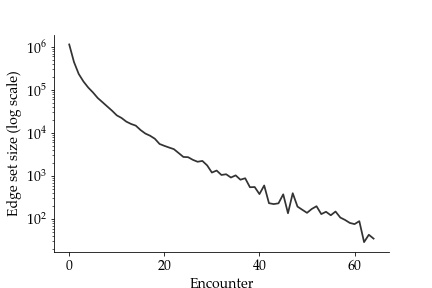
\includegraphics[scale=0.5]{encntr_edges.jpg}
    \caption{Edge set size for encounter graphs.}
    \label{fig:edge_dist}
\end{figure}

\begin{table}
    \caption{
      Top EHR features per category, common between degree and eigenvector centrality.
    }
    \label{tab:exp}
    \centering
    %
    \centering
    \label{tab:exp-synth}
    \begin{small}
    \begin{sc}
    \begin{tabular}{ll}
    \toprule
    Category                       & Top features by centrality \\
    \midrule
    Diagnoses                         & Ischemic stroke, High blood pressure, Long-term blood thinner use, \\ & Type-2 diabetes \\
    Medications                         & Heparin, Sodium chloride, Albuterol-ipratoropium, Eye drops\\
    Lab results                         & Glucose POC, Sodium Lvl, Glucose Lvl, BUN     \\
    Vital signs                            & SpO2 \%, Systolic blood pressure, Respiratory rate, Glasgow coma score     \\ 
    Orders                    & POC Glu, Auto Diff, CBC w/Auto Diff, Bill - Glu POCT, BMP \\
    \bottomrule
    \end{tabular}
    \end{sc}
    \end{small}
    \vskip -0.1in
\end{table}


\begin{figure}
    \centering
    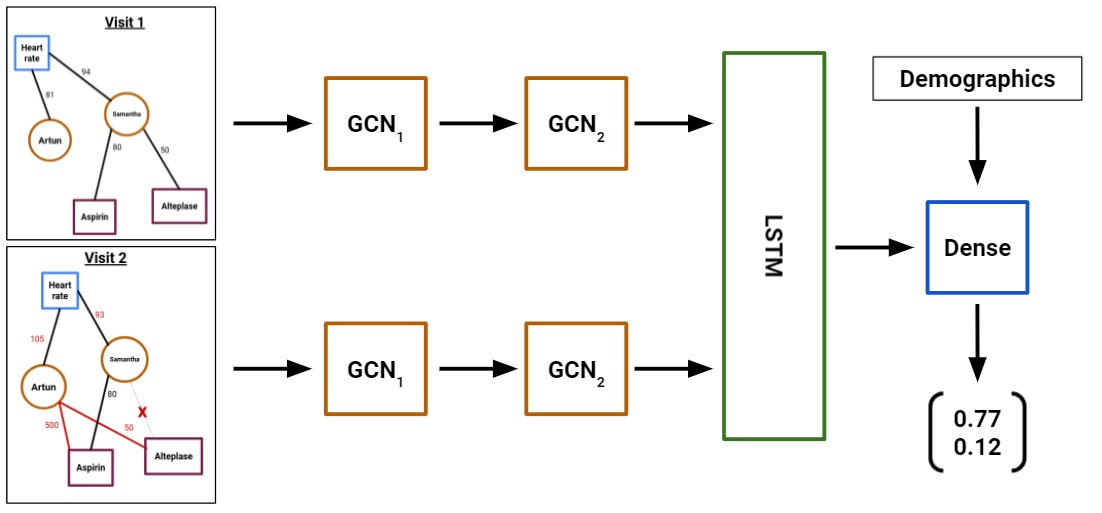
\includegraphics[scale=0.35]{horde_architecture.jpg}
    \caption{HORDE model architecture.}
    \label{fig:horde_arch}
\end{figure}

\subsection{HORDE model architecture}

As my primary model, I implemented the HORDE architecture (Lee et al., 2020) diagrammed in Figure 2. First, each encounter's graph is passed through the same multi-layer GCN to compute a per-encounter embedding for each node. As the shift operator, each GCN layer uses the symmetric normalized adjacency matrix $\textbf{A}^{sym} = \textbf{D}^{-\frac{1}{2}}\textbf{AD}^{-\frac{1}{2}}$,  such that each layer $k$ can be constructed as $\textbf{H}^{(k+1)} = \sigma(\textbf{A}^{sym}\textbf{H}^{(k)}\textbf{W})$ for inputs $\textbf{H}$, weights $\textbf{W}$, and activation function $\sigma$ (here, ReLU). Next, each patient node's embeddings are aggregated across encounters using long short-term memory (LSTM), a recurrent architecture that outputs a single embedding per node, describing how that node's encounter-level embeddings change over time. Finally, the LSTM embeddings are concatenated with time-invariant demographic features, and fed into a single fully-connected layer, which outputs the probability that the patient will have a recurrent stroke. For example, in Figure 2, three EHR features recorded over two encounters are used to predict recurrent stroke probability for two patients.

\subsection{HORDE benchmarking configuration}

In a deviation from the HORDE paper, I train the model in a supervised manner using cross-entropy loss, since it is only being leveraged for a single task. By default, I train HORDE with learning rate 0.0001, 325 epochs, 2 GCN layers with dimension 256, a 64-unit LSTM, 0.5 dropout rate, and balanced class weights. I implement all models using Tensorflow, but since the rights are owned by my sponsors at UTHealth, the code is not publicly available. 

For hyperparameter tuning and initial model selection, I create 80\% train / 10\% validation / 10\% test splits. All other results are obtained using 10-fold cross-validation, averaged over the last 25 epochs of each training. Since the dataset is significantly imbalanced (15\% positive), I use specificity, sensitivity and area under the precision-recall curve ($AUPRC$) as metrics. I also include $AUROC$ as a comparison metric for future work, although it is generally ill-suited for imbalanced data. Further, for AUC computation, the evaluation set is oversampled so that the stroke recurrence rate over the selected amount of time is equal to that for all 2019 patients. This is done to correct the imbalance induced by the fact that unlike negative samples, positive samples having a recurrent stroke $n$ months after the initial one can be included as having a stroke within the next $m$ months even if $n << m$, while negative samples occurring less than $m$ months ago must be filtered out, since it is not known for certain whether they had a recurrent stroke within $m$ months.


\section{HORDE model performance}

In this section, I provide performance metrics for the HORDE model under a variety of conditions, including time since initial stroke, initial stroke type, data availability, and recurrence window lengths.

\subsection{Model selection}

\begin{table}
    \caption{
      Performance of HORDE framework perturbations on stroke recurrence prediction task.
    }
    \label{tab:exp}
    \centering
    %
    \centering
    \label{tab:exp-synth}
    \begin{small}
    \begin{sc}
    \begin{tabular}{lrrr}
    \toprule
    Model                         & Specificity & Sensitivity & AUPRC \\
    \midrule
    Logistic regression                                & 1.00 & 0.00 & 0.12 \\
    SVM                                    & 0.24 & 0.96 & 0.22     \\
    HORDE                                  & 0.91 & 0.34 & \textbf{0.31}   \\
    HORDE (weight 1s higher)               & 0.79 & 0.45 & 0.29   \\
    HORDE (3 GCN layers)                   & 0.22 & 0.87 & 0.17   \\
    HORDE (first 5 encounters)             & 0.86 & 0.31 & 0.25   \\
    HORDE (first 2 encounters)             & 0.82 & 0.32 & 0.19   \\
    HORDE$_{agg}$                            & 0.71 & 0.48 & 0.15   \\
    \bottomrule
    \end{tabular}
    \end{sc}
    \end{small}

\end{table}

Table 4 compares the validation set performance of the HORDE framework to baseline models on all patient data, trained for 2000 epochs without time window restrictions. In addition to the standard HORDE model, I report performance using basic perturbations to the HORDE framework, modifying both the input graphs and model hyperparameters.

Generally, perturbations to the default HORDE framework's hyperparameters or data do not increase performance. Using a higher class weight for the positive samples improves sensitivity but greatly decreases sensitivity, for overall worse performance. Increasing the number of GCN layers causes the model to overfit, significantly reducing performance. Additionally, using only the first 5 or 2 (instead of all 65) encounters generally preserves sensitivity, reducing only specificity. Finally, training the HORDE model on a sum-aggregated, single-encounter version gives quite poor performance, implying that the temporal information between encounters is crucial to predicting stroke recurrence. Therefore, I selected the standard HORDE framework for use in future experiments.


\begin{table}
    \caption{
      HORDE model performance for various time window lengths.
    }
    \label{tab:exp}
    \centering
    %
    \centering
    \label{tab:exp-synth}
    \begin{small}
    \begin{sc}
    \begin{tabular}{lrrrrrr}
    \toprule
    Time window length & Samples & Pos. ratio & Spec. & Sens. & AUROC & AUPRC \\
    \midrule
    3 months & 427 & 0.09 & 0.72 & 0.42 & 0.64 & 0.16 \\
    6 months & 291 & 0.14 & \textbf{0.89} & 0.29 & 0.62 & 0.26 \\
    1 year & 136 & 0.25 & 0.82 & \textbf{0.66} & 0.74 & \textbf{0.55} \\
    \bottomrule
    \end{tabular}
    \end{sc}
    \end{small}

\end{table}



\subsection{Performance by time since initial stroke}

Next, I explore how the performance of the selected HORDE model varies with the length of time after the initial stroke at which recurrence status is evaluated. For this task, the model predicts whether a patient will have a recurrent stroke at any point in the $m$-month window after the initial stroke, using up to $m$ months of encounter data. The use of a time window for this problem is necessary because the dataset's patients are generally still alive, and had recent initial strokes. This means that it is impossible to conclusively say whether a negative sample patient will not ever have a recurrent stroke---they might still have one in the future. We can definitively state, however, whether the patient had a stroke in the next $m$ months after their initial stroke, as long as the initial stroke was at least $m$ months ago, or the patient had a recurrent stroke within $m$ months. Also, since our dataset is restricted to 2019-2020, using a longer recurrence window requires filtering out many negative samples; for example, a negative sample patient whose initial stroke occured on Dec. 1, 2020 could not be included for a 3-month time window, since it is unknown whether they had a recurrent stroke during Jan.-Feb. 2021 (window months 2 and 3).

Table 5 contains performance metrics for the HORDE model, trained over 3-month, 6-month, and 1-year time windows. Generally, performance improves as the length of the time window increases. This intuitively makes sense, since the more data is available on a patient, the better their current condition---and risk of recurrent stroke---can be understood. Further, the model's specificity is always significantly higher than its sensitivity. This is especially useful in a medical setting, as high specificity implies that any positive predictions the model makes are quite reliable. Therefore, patients the model identifies as having high recurrent stroke risk could be scheduled for additional preventative care, with a low risk of wasting these resources. For a 6-month time window, the model identifies almost $\frac{1}{3}$ of all high-risk patients with very high specificity ($AUPRC$ = 0.26); increasing the window length to 1 year doubles to $\frac{2}{3}$ ($AUPRC$ = 0.55), with only a minor decrease in specificity.


\subsection{Performance by initial stroke type}


\begin{table}
    \caption{
      Performance of HORDE model on 1-year time window, partitioned by initial stroke type.
    }
    \label{tab:exp}
    \centering
    %
    \centering
    \label{tab:exp-synth}
    \begin{small}
    \begin{sc}
    \begin{tabular}{lrrrrrr}
    \toprule
    Initial stroke type & Samples & Pos. ratio & Spec. & Sens. & AUROC & AUPRC \\
    \toprule
    All        & 255 & 0.25 & 0.82 & 0.66 & 0.74 & \textbf{0.55} \\
    \midrule
    AIS (Arterial ischemic)       & 164 & 0.25 & 0.80 & 0.66 & 0.72 & 0.55  \\
    ICH (Hemorrhage)        & 24 & 0.30 & 0.78 & 0.56 & 0.67 & 0.56 \\
    SAH (Subarachnoid hem.)        & 13 & 0.23 & 0.81 & 0.81 & 0.82 & \textbf{0.79}\\
    TIA (Transient ischemic)        & 19 & 0.24 & 0.92 & 0.73 & 0.82 & 0.75 \\
    Multi-type & 35 & 0.26 & 0.82 & 0.63 & 0.72 & 0.61 \\
    \midrule
    SAH, TIA, or Multi-type & 67 & 0.24 & 0.86 & 0.68 & 0.77 & \textbf{0.65} \\
    SAH or TIA & 32 & 0.22 & 0.91 & 0.78 & 0.84 & \textbf{0.77}\\
    \bottomrule
    \end{tabular}
    \end{sc}
    \end{small}
\end{table}

\begin{table}
    \caption{
      HORDE model performance for various data and recurrence window lengths.
    }
    \label{tab:exp}
    \centering
    %
    \centering
    \label{tab:exp-synth}
    \begin{small}
    \begin{sc}
    \begin{tabular}{llrrrrrr}
    \toprule
    Data window & Rec. window & Samples & Pos. ratio & Spec. & Sens. & AUROC & AUPRC \\
    \midrule
    < 1 month & 1 month & 193 & 0.07 & 0.29 & 0.11 & 0.19 & 0.02  \\
              & 3 months & 466 & 0.09 & 0.85 & 0.27 & 0.63 & 0.16 \\
              & 1 year & 268 & 0.25 & 0.59 & 0.59 & 0.60 & \textbf{0.40} \\
    \midrule
    1 month  & 3 months & 457 & 0.09 & 0.47 & 0.51 & 0.49 & 0.10 \\
             & 1 year & 128 & 0.25 & 0.73 & 0.55 & 0.65 & \textbf{0.43} \\
    \midrule
    3 months & 3 months & 222 & 0.09 & 0.48 & 0.54 & 0.50 & 0.12 \\
             & 1 year & 89 & 0.25 & 0.83 & 0.49 & 0.65 & \textbf{0.44}\\
    \midrule
    6 months & 1 month & 446 & 0.07 & 0.20 & 0.60 & 0.40 & 0.07 \\ % if time
             & 3 months & 102 & 0.09 & 0.53 & 0.45 & 0.45& 0.15 \\
             & 6 months & 101 & 0.14 & 0.75 & 0.26 & 0.45 & 0.21 \\
             & 1 year & 90 & 0.24 & 0.85 & 0.56 & 0.77 & \textbf{0.50} \\
             
    \bottomrule
    \end{tabular}
    \end{sc}
    \end{small}

\end{table}

A useful feature of my dataset is that each patient's initial stroke type is known at the time of recurrence prediction. Therefore, it is valid to partition patients by initial stroke type, and observe model performance on each. These results are described for the 1-year recurrence window in Table 6. Note that sample sizes are after oversampling, to represent a realistic patient distribution, and averaged across the 10 cross-validation folds.

On the most common initial stroke type, AIS, the model gives average performance, recovering $\frac{2}{3}$ of recurrent strokes with high specificity. However, the model gives significantly stronger performance on the two least common stroke types, SAH and TIA. Combining these two partitions into a single set, making up 13\% of patients, gives overall $AUPRC$ = 0.77, a very strong result. Additionally, since the model performs well on patients having multi-type initial strokes---the second-most common type---a larger high-performance subset can be created from TIA, SAH, and multi-type initial strokes, totaling 25\% of all patients. This subset has an overall $AUPRC$ = 0.65, with higher specificity and sensitivity compared to the set of all patients.  

The availability of initial stroke type data offers significant flexibility in deployment of this model. For example, if a hospital has limited preventative care resources, wasting these resource on false-positive predictions might be costly; therefore, they could apply the model to a small subset of patients for which results are especially reliable (e.g. SAH and TIA). Alternatively, if resources are not scarce, the slightly-larger (SAH, TIA, multi-type) subset could be used to increase coverage to more patients. Finally, if resources are abundant, the model could be applied to all patients.

\subsection{Performance by data and recurrence window lengths}

In addition to time since initial stroke and initial stroke type, it is also useful to evaluate how the model's performance is affected by the amount of data available and length of the recurrence window. Specifically, the model uses at least $d$ months of past encounter data (the \textit{data window}) to predict whether the patient will have a recurrent stroke in the next $r$ months (the \textit{recurrence window}). Note that $d+r=m$, the length of the time window described in \textbf{Section 6.2}, so this analysis is a more detailed exploration of the effects of time window length on model performance.

Table 7 describes how the HORDE model's performance varies for different data and recurrence window lengths. Interestingly, model performance seems to sharply increase with recurrence window length, and slightly increase with data window length; it appears as if a patient's condition can be captured well in the first few visits, but it is very difficult to determine when their next stroke will occur. Although exceptions exist in the data window length correlation, these are likely due to availability of training data; for example, <1 month of data outperforms 3 months of data for a 3-month recurrence window, but the <1 month dataset is twice as large. Based on these results, the model can be applied to patients with any amount of data with reasonable performance, but should only be used to predict long-term risk of recurrent stroke, as opposed to immediate concerns.

\section{HORDE variation architectures}


\begin{table}
    \caption{
      Hyperparameters varied for training HORDE variation architectures.
    }
    \label{tab:exp}
    \centering
    %
    \centering
    \label{tab:exp-synth}
    \begin{small}
    \begin{sc}
    \begin{tabular}{lrr}
    \toprule
    Architecture & Hidden layer dim. & Epochs \\
    \toprule
    HORDE & 256 & 325 \\
    HORDE$_L$ & 256 & 200 \\
    HORDE$_H$ & 128 & 250 \\
    HORDE$_{L+H}$ & 128 & 200 \\
    \bottomrule
    \end{tabular}
    \end{sc}
    \end{small}
    \vskip -0.1in
\end{table}

\begin{table}
    \caption{
      Performance of various architectures on 1-year time window.
    }
    \label{tab:exp}
    \centering
    %
    \centering
    \label{tab:exp-synth}
    \begin{small}
    \begin{sc}
    \begin{tabular}{llrrrrr}
    \toprule
    Patient subset & Architecture & Spec. & Sens. & AUROC & AUPRC \\
    \toprule
    All        & HORDE & 0.82 & 0.66 & 0.74 & 0.55 \\
               & HORDE$_L$ & 0.85 & 0.67 & 0.77 & 0.62 \\
               & HORDE$_H$ & 0.78 & 0.69 & 0.76 & 0.61 \\
               & HORDE$_{L+H}$ & 0.85 & 0.68 & 0.78 & \textbf{0.63} \\
    \midrule
    SAH, TIA, or Multi & HORDE & 0.86 & 0.68 & 0.77 & 0.65 \\
               & HORDE$_L$ & 0.89 & 0.70 & 0.82 & \textbf{0.72} \\
               & HORDE$_H$ & 0.77 & 0.72 & 0.79 & 0.69 \\
               & HORDE$_{L+H}$ & 0.86 & 0.71 & 0.83 & 0.69 \\

    \bottomrule
    \end{tabular}
    \end{sc}
    \end{small}
    \vskip -0.1in
\end{table}

For further benchmarking, I compare the standard HORDE architecture to two modified architectures: one using the Laplacian as the GCN shift operator, and one using a heterogeneous GCN layer. 

\subsection{Laplacian shift operator}

Prior spectral graph learning work, including Bruna et al. (2013) and Roddenberry, Glaze, and Segarra (2021) support using the graph Laplacian matrix as a GCN shift operator to give stronger performance than with the adjacency matrix, so I do the same with this task. The Laplacian $\textbf{L}$ is defined as $\textbf{L} = \textbf{D} - \textbf{A}$, where $\textbf{D}$ is the degree matrix and $\textbf{A}$ is the adjacency matrix. Specifically, I use the symmetric normalized Laplacian $\textbf{L}^{sym} = \textbf{D}^{-\frac{1}{2}}\textbf{LD}^{-\frac{1}{2}}$. The GCN layer is thus defined as $\textbf{H}^{(k+1)} = \sigma(\textbf{L}^{sym}\textbf{H}^{(k)}\textbf{W})$.


\subsection{Heterogeneous GCN}
Since the HORDE graph contains multiple types of nodes (namely, patient and feature nodes), I implemented a heterogeneous GCN layer, GCN$_H$, to explore whether this heterogeneity can be leveraged to learn more useful node representations. This layer trains two separate weight matrices, \textbf{ W}$_p$ and \textbf{W}$_f$, for patient and feature nodes respectively. Each node's convolution with its neighborhood is performed using the weight matrix corresponding to the node's type (patient or feature), allowing type-specific representations to be learned. First,  split both the input matrix \textbf{H} row-wise into \textbf{H}$_p$ and \textbf{H}$_f$, each containing all patient and feature nodes respectively. Then, the GCN$_H$ layer can be computed using $\textbf{H}^{(k+1)} = \sigma(\textbf{A}^{sym}(\textbf{H}_p^{(k)}\textbf{W}_p \mathbin\Vert \textbf{H}_f^{(k)}\textbf{W}_f))$, where $\mathbin\Vert$ represents vertical matrix concatenation.

\subsection{Performance comparison}

I train each of these models using the hyperparameters shown in Table 8, found through manual tuning on the 10\% validation set. Performance is evaluated on the 1-year time window. Also, I train the GCN hidden layers in HORDE$_H$ (computed using \textbf{W}$_p$ and \textbf{W}$_f$) with dimension 128, half the dimension of the 256-unit hidden layers in the standard HORDE GCN; this is to ensure that the same total number of parameters is used for each model.

As seen in Table 9, substituting either the Laplacian as the GCN shift operator (HORDE$_L$) or using a heterogeneous GCN layer (HORDE$_H$) improves model performance. Using both modifications together (HORDE$_{L+H}$) gives the best performance, with $AUPRC$ = 0.63 on all patients. Also, although HORDE$_L$ and HORDE$_H$ perform similarly on all patients, HORDE$_L$ performs notably better on the (SAH, TIA, multi-type) subset described previously, outperforming all other architectures. Further, HORDE$_L$ and HORDE$_H$ both train faster than the standard HORDE model, with Laplacian-shift architectures requiring only 200 epochs to produce good results. Overall, HORDE$_L$ appears to be the best architecture, since it has the best performance on the (SAH, TIA, multi-type) subset and fewest training epochs required, with similar performance to HORDE$_{L+H}$ on all patients. 

\section{Conclusion}

This project demonstrates a successful application of the HORDE framework, and graph learning in general, to recurrent stroke prediction. The best model gives $AUPRC$ > 0.6 and $AUROC$ > 0.75, and can reliably identify over $\frac{2}{3}$ of high-risk stroke patients for a 1-year time window. Further, selecting patients by initial stroke type allows for $AUPRC$ > 0.7 and $AUROC$ > 0.8 on a 25$\%$ subset of patients. I also demonstrate that the length of the recurrence window more dramatically affects model performance than the amount of available data, and that variations on the HORDE architecture inspired by both spectral graph theory and the HORDE graph's heterogeneous structure can improve performance. These results are especially promising given both the documented unreliability of EHRs (Lee et al., 2020) and the availability of both clinical note and brain scan datasets, which will be incorporated in future work to further improve results.

This model can be leveraged by hospitals to identify patients at high risk of recurrent stroke, for which preventative care could have significant impact. Further, the ability to know which patients are not at risk of recurrent stroke, and therefore need less preventative care, will help hospitals more efficiently distribute their medical resources. Overall, this work can be leveraged to reduce the rate of recurrent strokes, ultimately saving the lives of stroke patients worldwide.



% \begin{table}
%     \caption{
%       Performance of HORDE model on 1-year window, for notable patient subsets by initial stroke type. Val set negatives upsampled to 0.25 (overall 1-year recurrence ratio)
%     }
%     \label{tab:exp}
%     \centering
%     %
%     \centering
%     \label{tab:exp-synth}
%     \begin{small}
%     \begin{sc}
%     \begin{tabular}{lrrrrrr}
%     \toprule
%     Initial stroke type   & Samples & Pos. ratio & Spec. & Sens. & AUROC & AUPRC \\
%     \toprule
%     All        & 220 & 0.25 & 0.83 & 0.60 & 0.76 & \textbf{0.55} \\
%     \midrule
%     AIS (Arterial ischemic stroke)       & 141 & 0.26 & 0.81 & 0.58 & 0.74 & 0.50  \\
%     ICH (Intracerebral hemorrhage)        & 21 & 0.43 & 0.83 & 0.67 & 0.77 & 0.81 \\
%     SAH (Subarachnoid hemmorhage)        & 16 & 0.13 & 0.86 & 0.00 & 0.71 & 0.27\\
%     TIA (Transient ischemic attack)        & 19 & 0.05 & 1.00 & 1.00 & 1.00 & 1.00 \\
%     Multi-type & 23 & 0.30 & 0.75 & 0.71 & 0.83 & 0.74 \\
%     \midrule
%     ICH, TIA, or Multi-type & 63 & 0.27 & 0.87 & 0.71 & 0.81 & \textbf{0.72} \\
%     \bottomrule
%     \end{tabular}
%     \end{sc}
%     \end{small}
%     \vskip -0.1in
% \end{table}



% \begin{table}
%     \caption{
%       HORDE metrics on samples w/less than X months of data, predicting status at end of X months. Val data negatives oversampled to have ratio 0.25.
%     }
%     \label{tab:exp}
%     \centering
%     %
%     \centering
%     \label{tab:exp-synth}
%     \begin{small}
%     \begin{sc}
%     \begin{tabular}{llllllllll}
%     \toprule
%     & Spec. & & & Sens. & & & AUPRC & & \\
%     Initial stroke type & 3 mo. & 6 mo. & 1 yr. & 3 mo. & 6 mo. & 1 yr. & 3 mo. & 6 mo. & 1 yr. \\
%     \midrule
%     All & 0.96 & 0.95 & 0.83 & 0.16 & 0.28 & 0.60 & 0.40 & 0.56 & 0.55 \\
%     ICH, TIA, or Multi-type & 0.94 & 0.95 & 0.87 & 0.25 & 0.38 & 0.71 & 0.41 & 0.73 & 0.72 \\

%     \bottomrule
%     \end{tabular}
%     \end{sc}
%     \end{small}

% \end{table}

\section{References}
{
\small

[1] Aarnio, K., Haapaniemi, E., Melkas, S., Kaste, M., Tatlisumak, T., and Putaala, J. (2014). Long-Term Mortality After First-Ever and Recurrent Stroke in Young Adults. {\it Stroke}, 45, 2670-2676.

[2] Abedi, V., Avula, V., Chaudhary, D., Shahjouei, S., Khan, A., Griessenauer, C. J., Li, J., et al. (2021). Prediction of Long-Term Stroke Recurrence Using Machine Learning Models. Journal of Clinical Medicine, 10(6), 1286. MDPI AG. 

[3] Hamilton, W., Ying, R., Leskovec, J. (2017). Inductive Representation Learning on Large Graphs. {\it CoRR}, 1706, 2216.

[4] Hung, L. C., Sung, S. F., Hu, Y. H. (2020). A Machine Learning Approach to Predicting Readmission or Mortality in Patients Hospitalized for Stroke or Transient Ischemic Attack. {\it Applied Sciences}, 2020(10), 6337.

[5] National Institutes of Health (2019). Stroke. {\it National Heart, Lung, and Blood Institute.}

[6] Lee, D., Jiang, X., Yu, H. (2020). Harmonized representation learning on dynamic EHR graphs. Journal of Biomedical Informatics, 106, 1034216. 

[7] Roddenberry, T. M., Glaze, N., Segarra, S. (2021). Principled Simplicial Neural Networks for Trajectory Prediction. {\it International Conference on Machine Learning}, 2102, 10058.

[8] Roth, Gregory A., et al. (2018). Global, regional, and national age-sex-specific mortality for 282 causes of death in 195 countries and territories, 1980–2017. {\it The Lancet}, 392(10159), 1736-1788.

[9] Wang, X., Ji, H., Shi, C., Wang, B., Ye, Y., Cui, P., Yu, P. (2019). Heterogeneous Graph Attention Network. {\it The World Wide Web Conference}, 2020, 2022-2032.

\end{document}